\begin{figure*}[tbp]
  \centering
  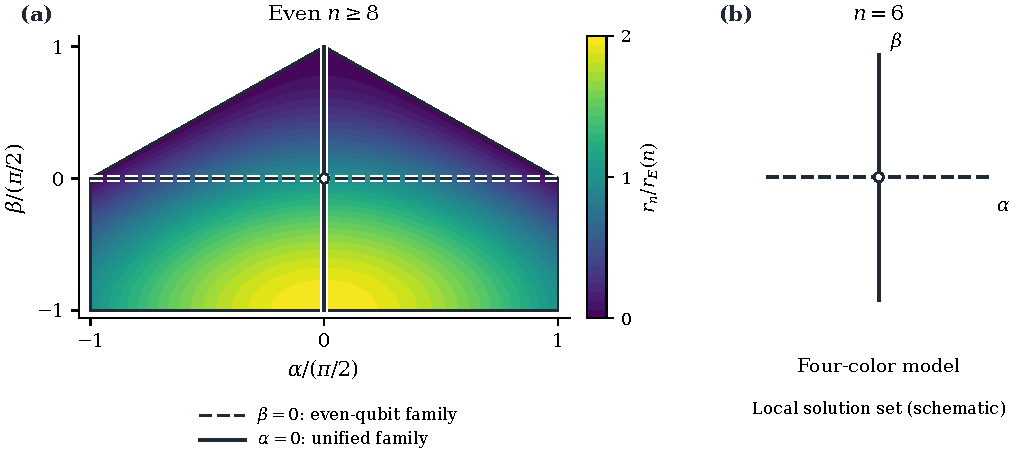
\includegraphics[width=\textwidth]{figures/fig2_embedding.pdf}
  \caption{Two exact sections of the even-qubit mother family.
  (a) The domain $\Omega$ for even $n\geq8$, colored by $r_n/r_E(n)=\cos\alpha-\sin\beta$.
  The dashed section $\beta=0$ recovers the prior even-qubit family, and the solid section $\alpha=0$ recovers the unified enhanced family, in each case column by column.
  The open circle marks the common base point.
  (b) Schematic local solution set at $n=6$ in the four-joint-color model with an independent zero-string phase: the two branches cross at the base point. Plotting code was prepared with OpenAI Codex (GPT-6) assistance and checked against the stated formulas.}
  \label{fig:embedding}
\end{figure*}
